\section{Die Benutzerschnittstelle}
	In diesem Abschnitt dieses Kapitels wird auf die Implementierung der Benutzerschnittstelle eingegangen. Wie schon bereits im SRS erwähnt handelt es sich bei der Benutzerschnittstelle um die grafische Oberfläche der Android App. Dafür wird zunächst auf die Umsetzung eingegangen und abschließend die Auswertung der Benutzeroberfläche mit einem Usability Test behandelt.
		
	\subsection{Die Umsetzung}	
		Um die ergonomie zu erhöhen kann der linke joystick i einem festgelegten bereich überall angelegt werden
		
		Da es sich um KOmponenten handelt die immer da sein müssen wurde sich für das normale UI Screen Space - OVerlay ausgewählt
		
		\begin{figure}[htbp]
			\centering 
			\label{alwaysOnUI}
			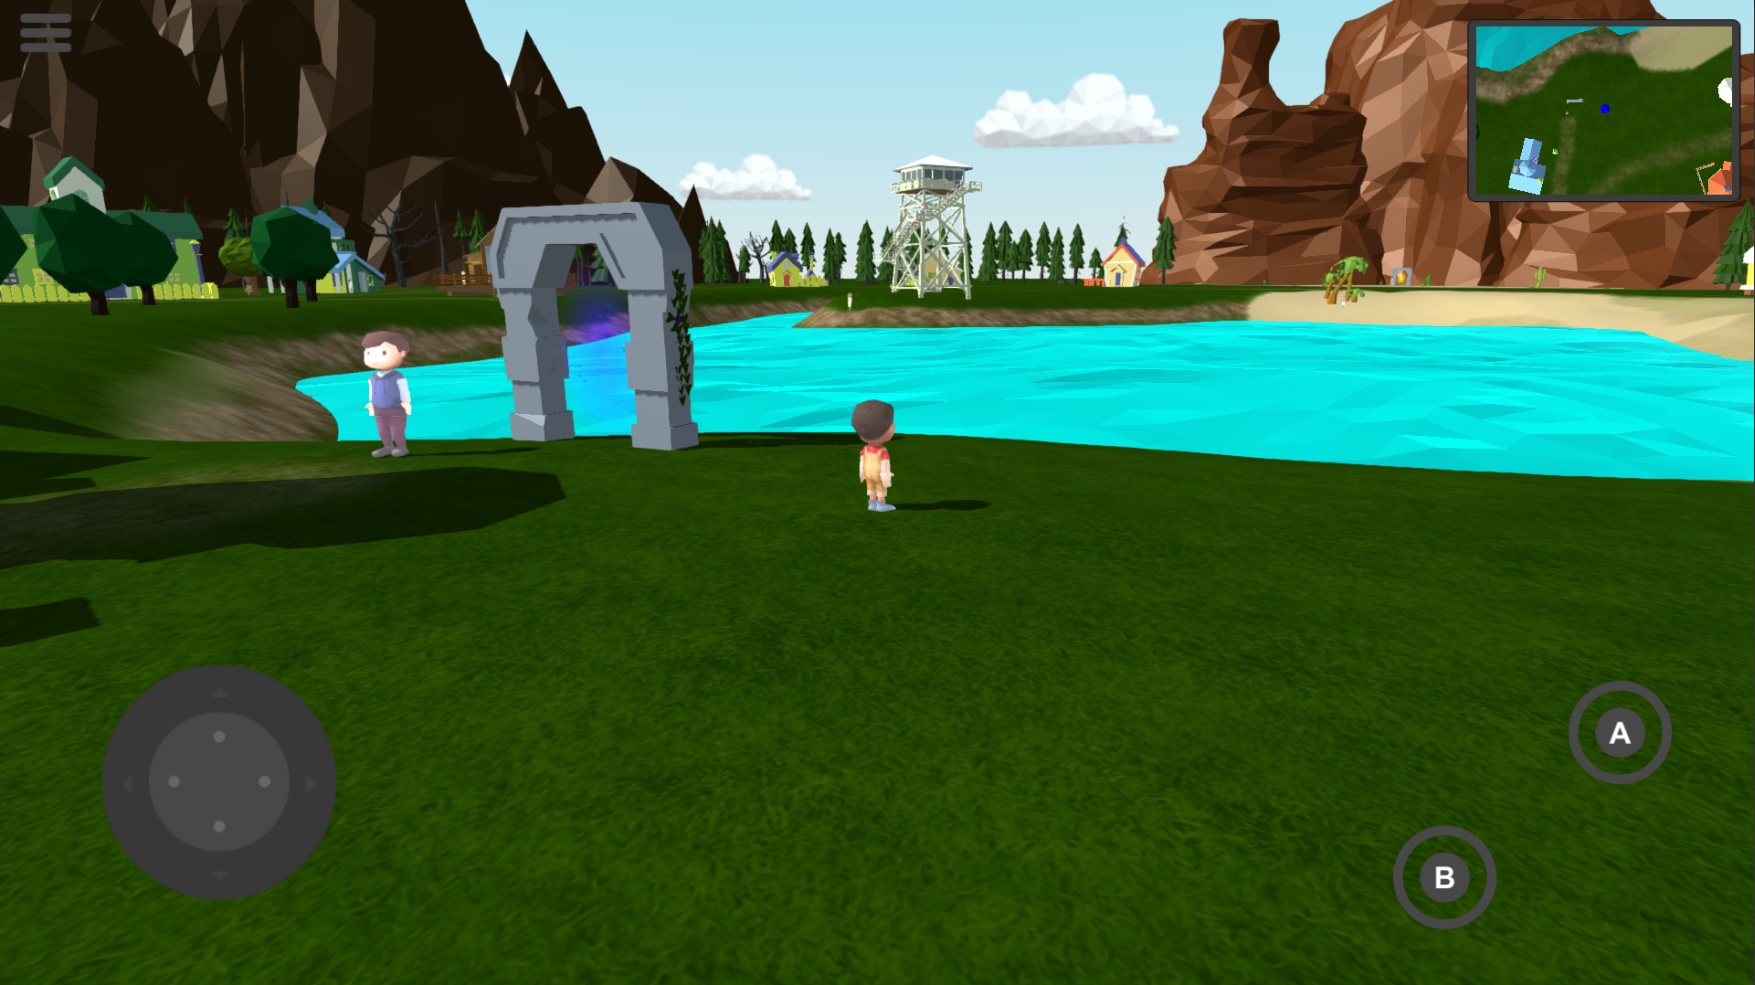
\includegraphics[width=13cm]{pics/alwaysOnUI.png}
			\caption{User Interface: Head-Up Display}
		\end{figure}
	
		\begin{figure}[htbp]
			\centering 
			\label{userInterfaces}
			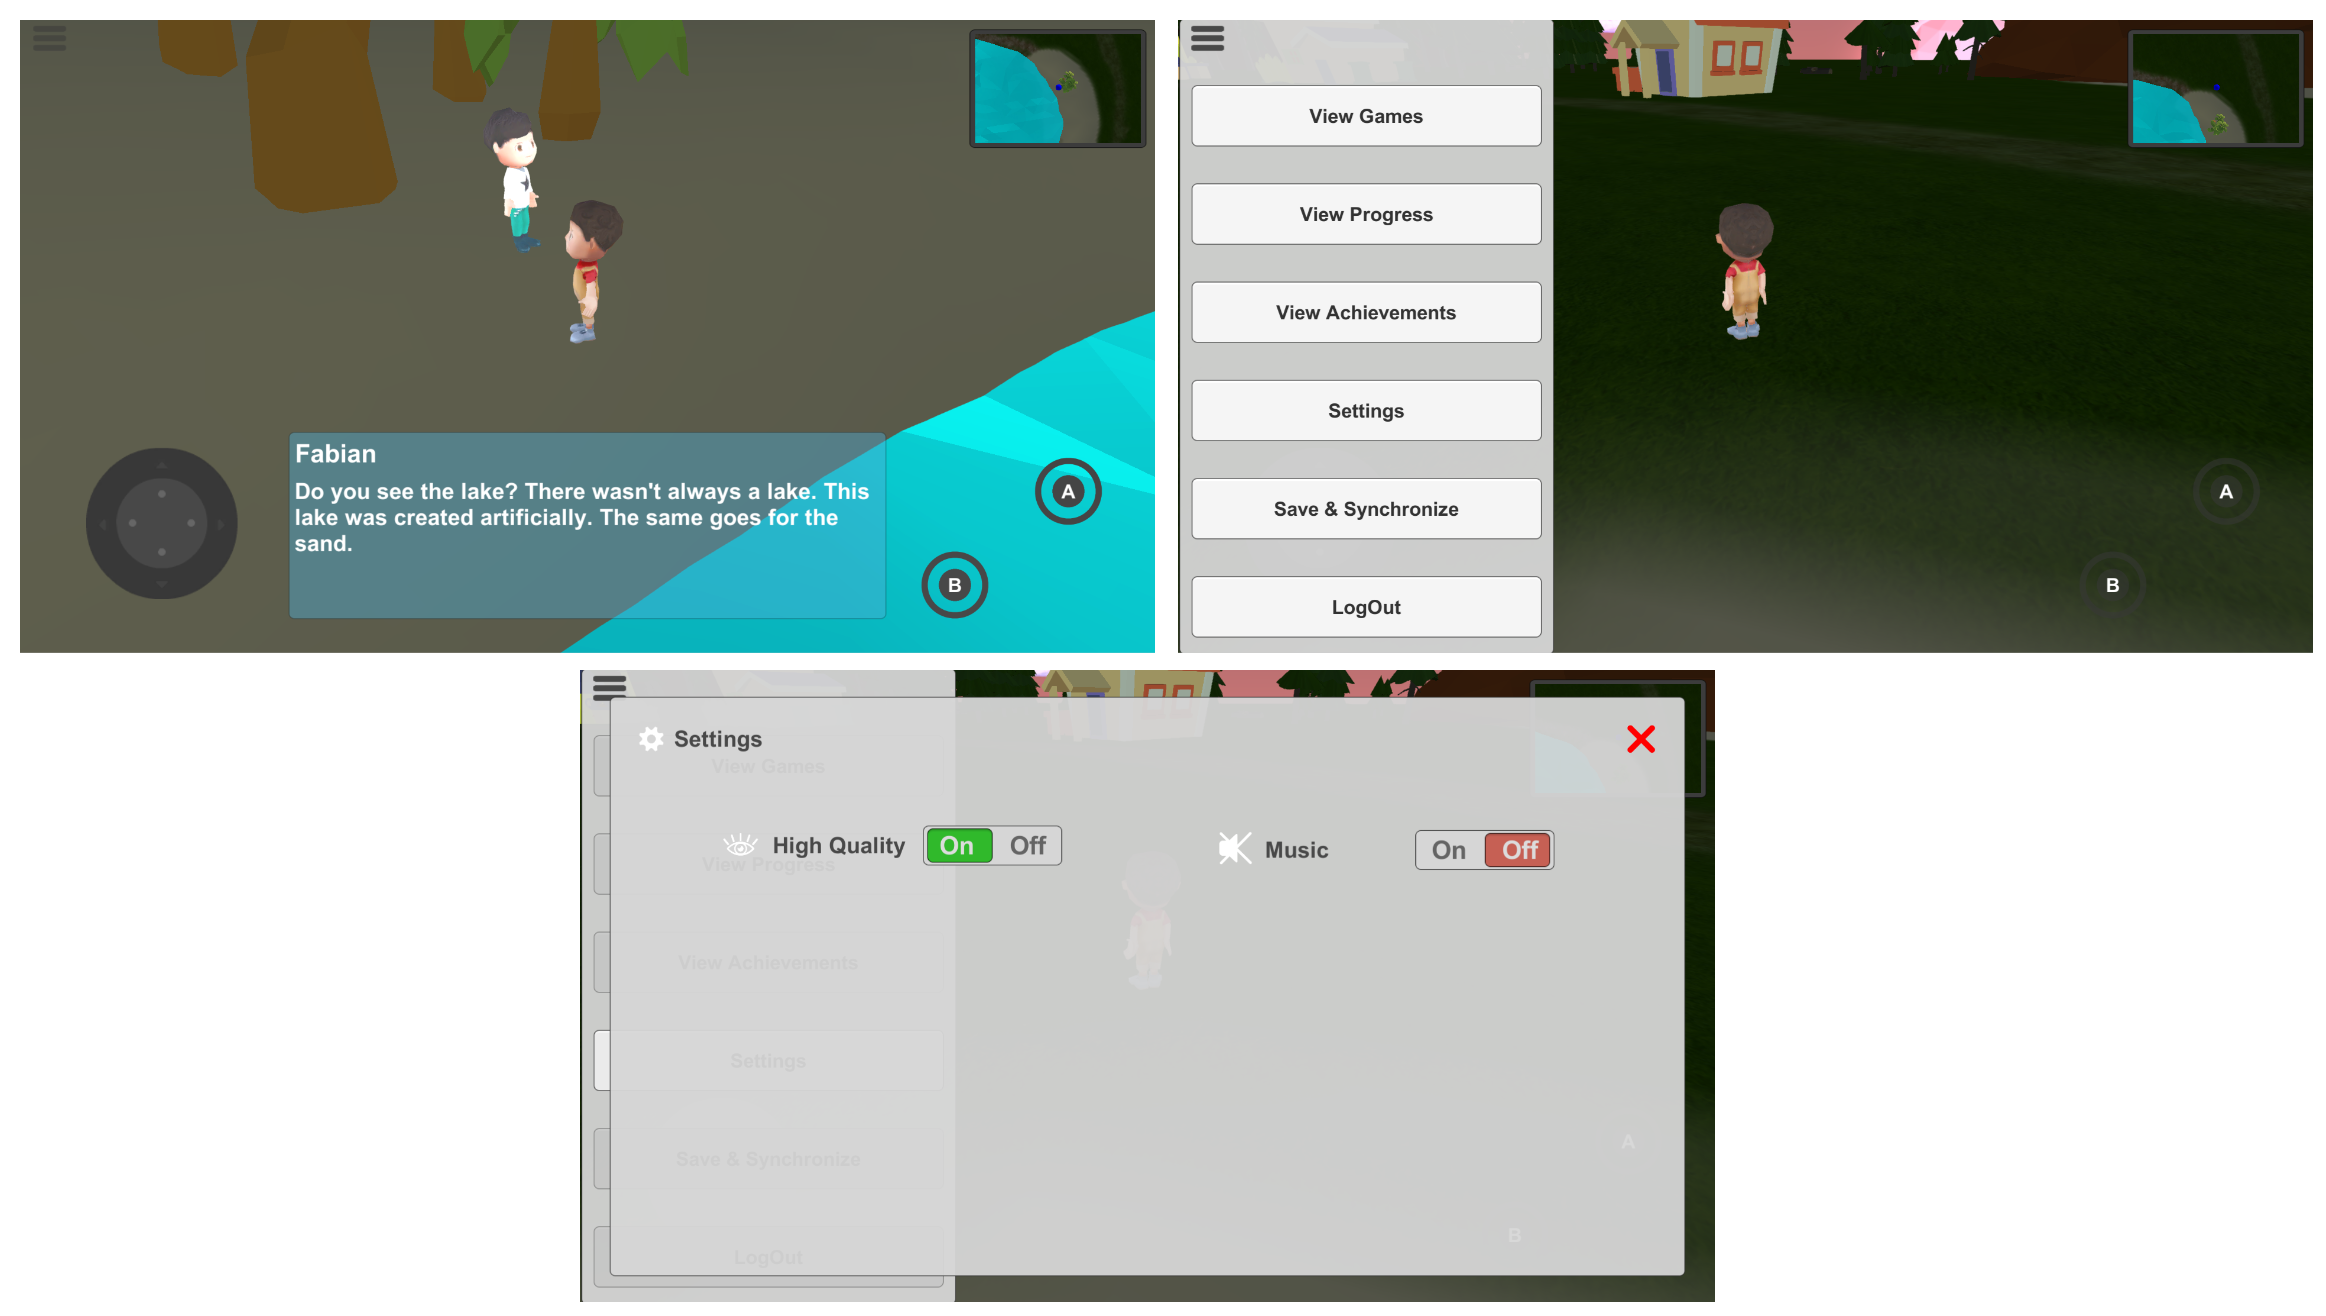
\includegraphics[width=\textwidth]{pics/userInterface.png}
			\caption{User Interfaces: Kommunikation, Menu und Einstellungen-Fenster}
		\end{figure}
	
		Menu fenster bildet die erste Dialogebene nach der Startebene. Nach diesem gibt es noch eine weitere Ebene. dieser Dialog dient zum Abbrechen, warnt vor bevorstehenden Aktionen. Die maximale Dialogebene ist also 2. 

		\begin{figure}[htbp]
			\centering 
			\label{RegisterUI}
			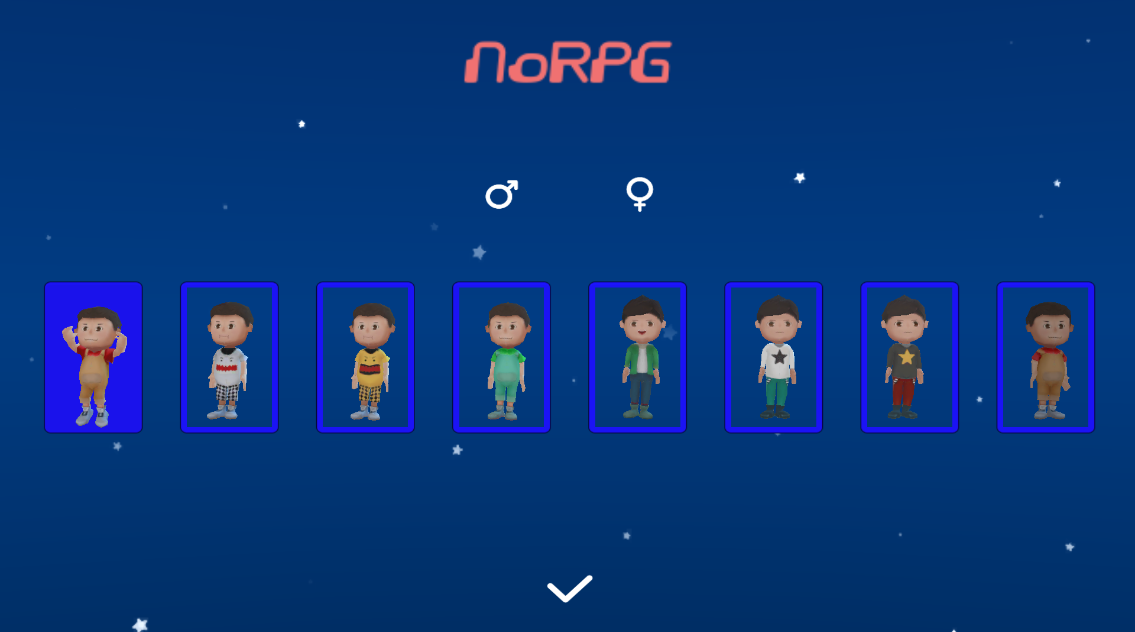
\includegraphics[width=13cm]{pics/RegisterUI.png}
			\caption{User Interface: Registrierung}
		\end{figure}

	
	\subsection{Usability Test}
		Usability TEst faken? Kinder + Jugendliche --> Katalog mit Bewertung
		Summativer TEst: Nach der Entwicklung, fertiges Produkt vor Auslieferung umfangreiche Studie
	
		Benutzerprofiele, Szenarien, Umfang, Zeitraum (3 Tage) 
	
		TEstutensilien: Prerelease version der APp und eigene Software
		Testart: Remotetest (vor und nachteile zu anderen)